\documentclass{article}
\usepackage{geometry}
\usepackage{ragged2e}
\usepackage{indentfirst}
\usepackage{listings}
\usepackage{xcolor} % for setting colors
\usepackage[justification=centering]{caption}
\usepackage{graphicx,wrapfig}
\usepackage{float}
\usepackage{xepersian}
% \settextfont{Yas}
\settextfont[BoldFont={XB Yas Bd}, ItalicFont={XB Yas It}, BoldItalicFont={XB Yas BdIt}, Extension = .ttf]{XB Yas}
\usepackage{setspace}
\usepackage{listings}

\geometry{a4paper,
 total={170mm,257mm},
 left=30mm,
 right=30mm,
 top=20mm,
 bottom=40mm
 }

\definecolor{dkgreen}{rgb}{0,0.6,0}
\definecolor{gray}{rgb}{0.5,0.5,0.5}
\definecolor{mauve}{rgb}{0.58,0,0.82}

\lstset{frame=tb,
  language=Java,
  aboveskip=3mm,
  belowskip=3mm,
  showstringspaces=false,
  columns=flexible,
  basicstyle={\small\ttfamily},
  numbers=none,
  numberstyle=\tiny\color{gray},
  keywordstyle=\color{blue},
  commentstyle=\color{dkgreen},
  stringstyle=\color{mauve},
  breaklines=false,
  breakatwhitespace=true,
  tabsize=4
}

\doublespacing
\makeatletter
\let\footnoteruleA=\right@footnoterule
\let\Afootnoterule=\right@footnoterule
\makeatother
\rightfootnoterule

\title{\textbf{توضیحات فاز اول پروژه‌ی داده‌کاوری}}
\author{محمد کاهانی، علی گلدانی}
\date{\parbox{\linewidth}{\centering
    عنوان پایگاه داده: SAP\endgraf
    \today\endgraf
    }}

\begin{document}
    \maketitle

    \begin{large}
        \section{شرح کلی دیتاست}
        SAP یک دیتاست آموزشی می‌باشد که از یک سیستم مدیریت آموزش به نام Kalboard-360 گردآوری شده است.
        این سیستم با هدف تسریع فرایند یادگیری، با استفاده از تکنولوژی‌های روز طراحی شده است و
        امکان دسترسی همگام‌سازی شده به منابع آموزشی را از طریق هر دستگاه متصل به اینترنت، به کاربران می‌دهد.

        این مجموعه داده از طریق یک ابزار ثبت فعالیت کاربران تهیه شده است. این ابزار رابط کابری تجربه (xAPI) نام دارد.
        این ابزار امکان نظارت بر روی نحوه‌ی پیشرفت یادگیری کاربران را از طریق ثبت فعالیت‌هایی مانند خواندن یک مقاله یا مشاهده‌ی یک ویدیو فراهم می‌کند.
        این ابزار به مسئولین کمک می‌کند تا بتوانند با تحلیل روند استفاده و پیشرفت کاربران، یک تجربه‌ی آموزشی را توصیف کنند.
        این مجموعه‌داده شامل ۴۸۰ دانش‌آموز و ۱۶ ویژگی در رابطه باآن‌هاست. این ویژگی‌ها در ۳ دسته‌ی کلی طبقه‌بندی می‌شوند:
        \begin{enumerate}
            \item اطلاعات جمعیتی مانند جنسیت و ملیت
            \item ویژگی‌های مربوط به سابقه‌ی تحصیلی مانند مقطع تحصیلی، سطح نمره و کلاس دانشجو
            \item ویژگی‌های رفتاری مانند تعداد دفعاتی که دانش‌آموز دستش را در کلاس بالا برده‌است، میزان استفاده از منابع درسی، پاسخگویی به پرسشنامه‌ها توسط والدین و رضایت از مدرسه
        \end{enumerate}
        دانش‌آموزان بر اساس نمره‌ی کل آن‌ها به سه بازه‌ی عددی تقسیم می‌شوند:
        \begin{itemize}
            \item \textbf{سطح پایین}: نمرات در بازه‌ی ۰ تا ۶۹
            \item \textbf{سطح متوسط}: نمرات در بازه‌ی ۷۰ تا ۸۹
            \item \textbf{سطح بالا}: نمرات در بازه‌ی ۹۰ تا ۱۰۰
        \end{itemize}

        \newpage
        \textbf{توضیح ویژگی‌های مجموعه‌داده:}
        \begin{center}
            \begin{tabular}{ | p{40mm} | p{100mm} | }
                \hline
                {\textbf{ویژگی}} & 
                {\textbf{توصیف}} \\
                \hline
                gender & جنسیت دانش‌آموز \\
                \hline
                Nationality & ملیت دانش‌آموز \\
                \hline
                PlaceofBirth & محل تولد دانش‌آموز \\
                \hline
                ‌StageId & مقطع تحصیلی دانش‌آموز \\
                \hline
                GradeId & سال تحصیلی دانش‌آموز \\
                \hline
                SectionId & کلاسی که دانش‌آموز در آن است \\
                \hline
                Topic & موضوع درس \\
                \hline
                Semester & نیم‌سال تحصیلی \\
                \hline
                Relation & پدر یا مادر مسئول دانشجو \\
                \hline
                raisedhands & میزان دفعاتی که دانش‌آموز دستش را در کلاس بالا برده است \\
                \hline
                VisitedResources & تعداد دفعاتی که دانش‌آموز منابع درس را مشاهده کرده است \\
                \hline
                AnnouncementsView & تعداد دفعاتی که دانش‌آموز اعلانات جدید را چک می‌کند \\
                \hline
                Discussion & تعداد دفعاتی که دانش‌آموز در گروه‌های مباحثه شرکت کرده‌است \\
                \hline
                ParentAnsweringSurvey & این که پدر یا مادر دانش‌آموز به پرسش‌نامه‌های مدرسه پاسخ داده است یا خیر \\
                \hline
                ParentschoolSatisfaction & این که پدر یا مادر از مدرسه رضایت داشته‌اند یا خیر \\
                \hline
                StudentAbsenceDays & این که دانش‌آموز بیش از ۷ جلسه غیبت داشته‌است یا خیر \\
                \hline
                Class & طبقه‌بندی دانش‌آموز بر اساس نمره‌ی کل \\
                \hline
            \end{tabular}
        \end{center}

        \newpage
        \section{پیش‌پردازش داده‌ها}
        \subsection{Cleaning Data}
        
        \begin{figure}[h]
            \centering
            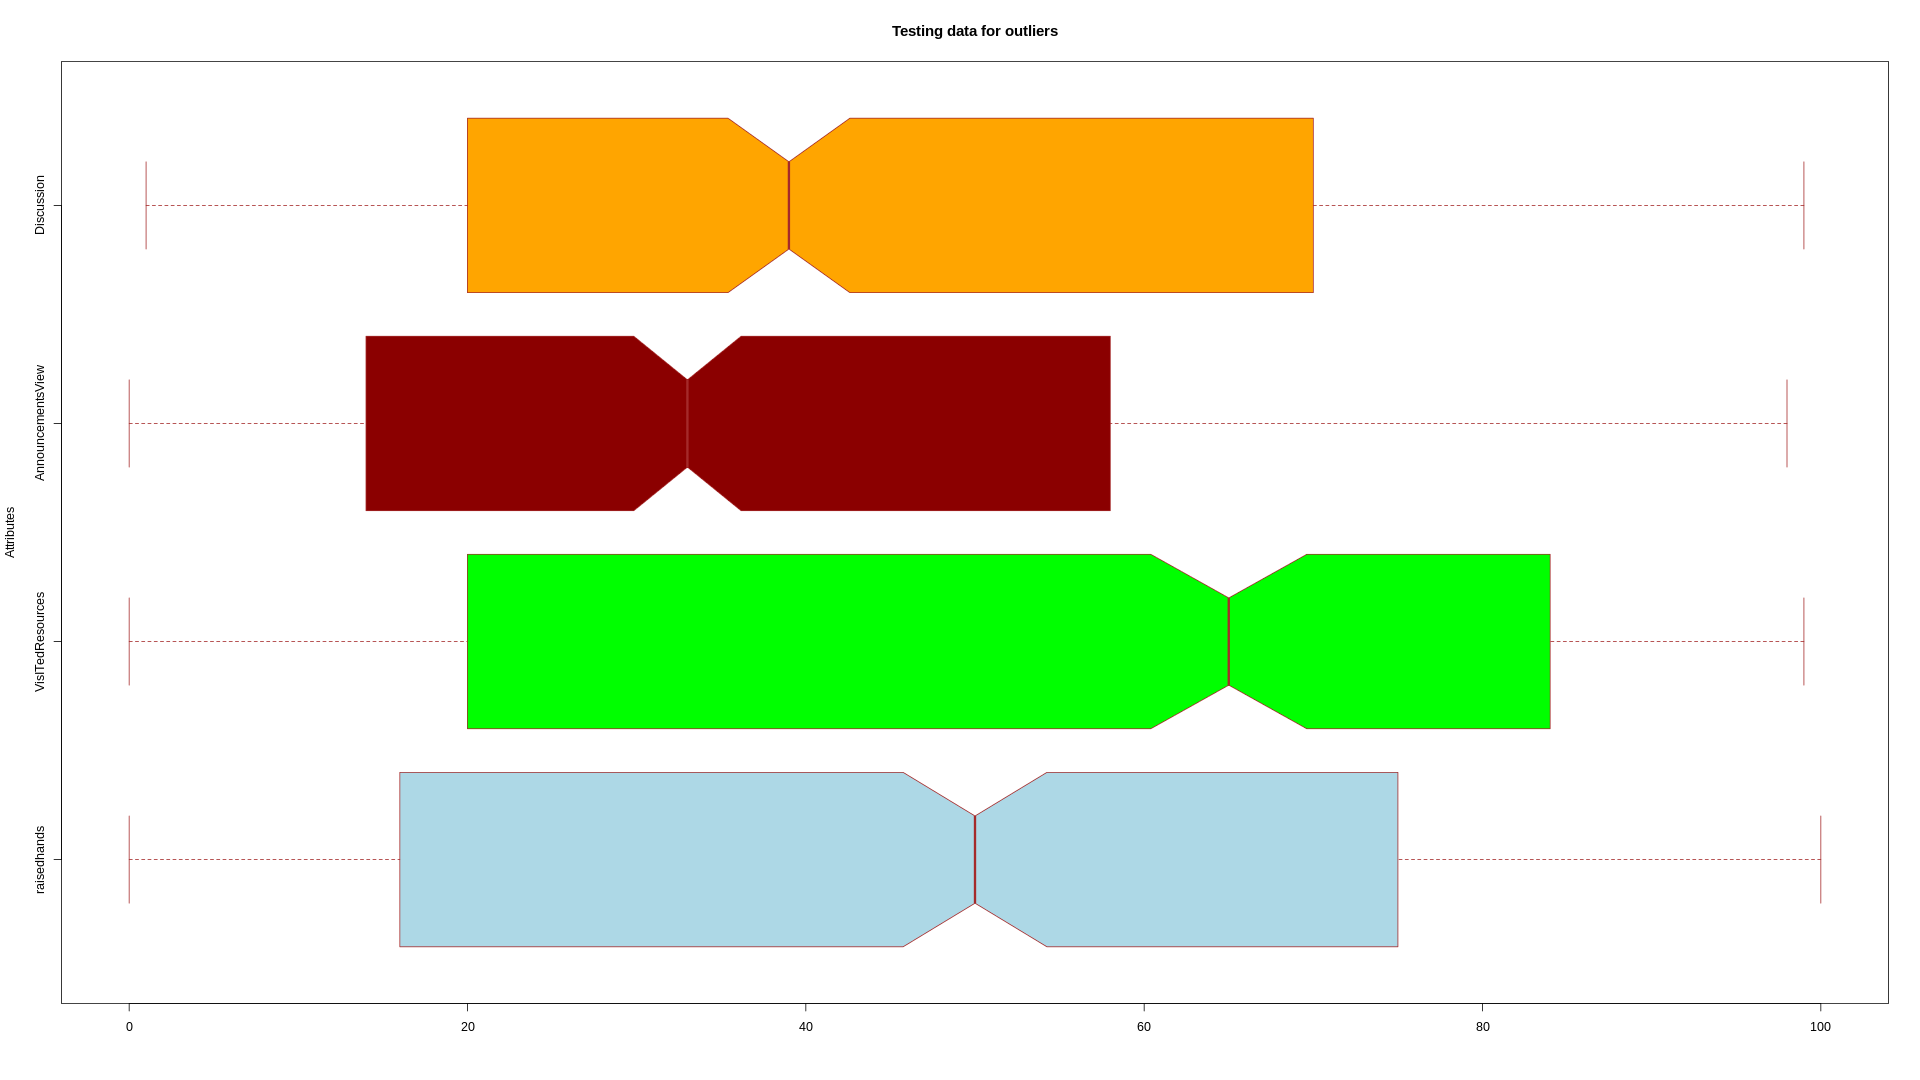
\includegraphics[width=1\textwidth]{images/boxplot.png}
            \caption{Diagram BoxPlot}
            \label{fig:boxplot}
        \end{figure}
        
        با رسم BoxPlot در شکل \ref{fig:boxplot} متوجه می‌شویم که داده‌ها بدون مقادیر نویز هستند.
\end{large}

	 
\end{document}